\begin{figure}[h]
	\centering
	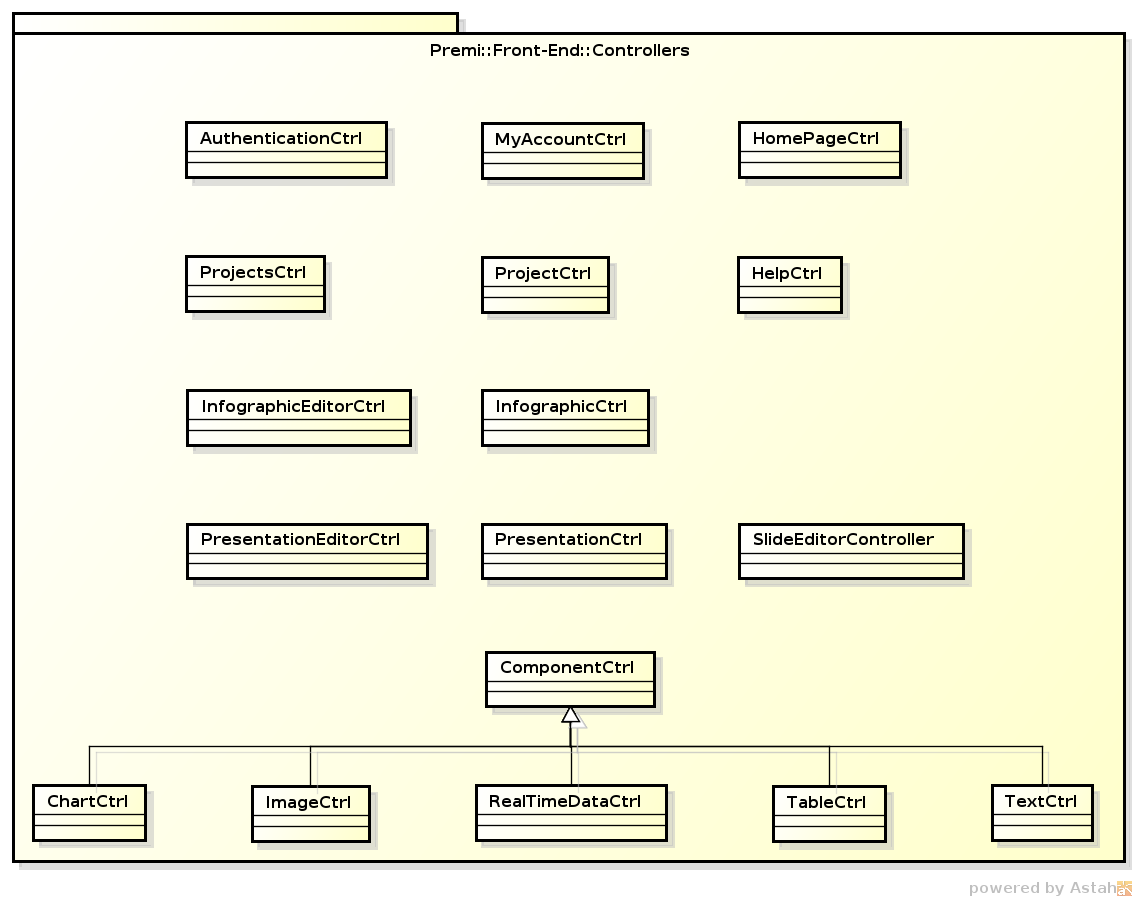
\includegraphics[width=0.7\linewidth]{img/premi_front_end_controllers}
	\caption[Premi::Front-End::Controllers]{Premi::Front-End::Controllers}
\end{figure}
Il package gestisce i controller del front-end dell'applicazione. Comunica con il model, le view e i service della struttura per gestire tutte le operazioni tra di essi. Fa comunicare le view con il model per rendere visibili gli aggiornati effettuati con quest'ultimo e viceversa, aggiorna il model con le informazioni provenienti dalla view. Richiama inoltre i service per comunicare con il back-end e caricare o salvare quindi i dati nel database.
\newpage

\subsubsection{ComponentController}
      \paragraph{Descrizione}
	Il controller ComponentController si occupa della costruzione e gestione dei componenti in una slide.
	
	\paragraph{Utilizzo}
	Questa classe viene utilizzata per consentire all'utente di aggiungere, modificare o rimuovere un componente in una slide.
	
	\paragraph{Attributi}
	\begin{itemize}
		\item \textbf{-\$scope: Object}:\\
				Campo dati contenente un riferimento all'oggetto \$scope creato da Angular, viene utilizzato come mezzo di comunicazione tra il controller e la view. Contiene gli oggetti che definiscono il model dell'applicazione.
	\end{itemize}
	
	\paragraph{Metodi}
	\begin{itemize}
	\item \textbf{+getX():Double}:\\
		Metodo che restituisce la distanza dal bordo sinistro del canvas utilizzata per l'ancoraggio dell'oggetto selezionato;
	\item \textbf{+getY():Double}:\\
		Metodo che restituisce la distanza dal bordo superiore del canvas utilizzata per l'ancoraggio dell'oggetto selezionato;
	\item \textbf{+getHeigth():Double}:\\
		Metodo che restituisce l'altezza dell'oggetto selezionato;
	\item \textbf{+getWidth():Double}:\\
		Metodo che restituisce la larghezza dell'oggetto selezionato;
	\item \textbf{+getExtraFields():JSON}:\\
		Metodo che restituisce un oggetto JSON con le informazioni aggiuntive dell'oggetto selezionato;
	\item \textbf{+getAngle():Double}:\\
		Metodo che restituisce l'angolo di rotazione dell'oggetto selezionato;
	\item \textbf{+getScaleX():Double}:\\
		Metodo che restituisce il livello di zoom applicato alla larghezza dell'oggetto selezionato;
	\item \textbf{+getScaleY():Double}:\\
		Metodo che restituisce il livello di zoom applicato all'altezza dell'oggetto selezionato;
	\item \textbf{+setX(\textit{value}:Double):void}:\\
		Metodo che permette di impostare la distanza dal bordo sinistro del canvas utilizzata per l'ancoraggio dell'oggetto selezionato al valore \textit{value};
	\item \textbf{+setY(\textit{value}:Double):void}:\\
		Metodo che permette di impostare la distanza dal bordo superiore del canvas utilizzata per l'ancoraggio dell'oggetto selezionato al valore \textit{value};
	\item \textbf{+setHeigth(\textit{value}:Double):void}:\\
		Metodo che permette di impostare l'altezza dell'oggetto selezionato al valore \textit{value};
	\item \textbf{+setWidth(\textit{value}:Double):void}:\\
		Metodo che permette di impostare la larghezza dell'oggetto selezionato al valore \textit{value};
	\item \textbf{+setExtraFields(\textit{obj}:JSON):void}:\\
		Metodo che permette di impostare le proprietà aggiuntive dell'oggetto selezionato prendendo i valori dall'oggetto JSON \textit{obj} passato per parametro;
	\item \textbf{+setAngle(\textit{value}:Double):void}:\\
		Metodo che permette di impostare l'angolo di rotazione dell'oggetto selezionato al valore \textit{value};
	\item \textbf{+setScaleX(\textit{value}:Double):void}:\\
		Metodo che permette di impostare il livello di zoom applicato alla larghezza dell'oggetto selezionato al valore \textit{value};
	\item \textbf{+setScaleY(\textit{value}:Double):void}:\\
		Metodo che permette di impostare il livello di zoom applicato all'altezza dell'oggetto selezionato al valore \textit{value}.
	\end{itemize}
	\paragraph{Relazioni con altre classi}
	\begin{itemize}
	 \item OUT: \textbf{SlideEditorController}:\\
		Il controller SlideEditorController utilizza ComponentController per la gestione dei componenti al fine di costruire la slide.
	\end{itemize}


\subsubsection{HelpController}
      \paragraph{Descrizione}
	Il controller HelpController gestisce i meccanismi di aiuto ll'utente.
	
	\paragraph{Utilizzo}
	Questa classe viene utilizzata per gestire le informazioni e la logica di erogazione degli aiuti all'utente sotto forma di suggerimenti(tips) esplicativi delle funzionalità.
	
	\paragraph{Attributi}
	\begin{itemize}
		\item \textbf{-\$scope: Object}:\\
				Campo dati contenente un riferimento all'oggetto \$scope creato da Angular, viene utilizzato come mezzo di comunicazione tra il controller e la view. Contiene gli oggetti che definiscono il model dell'applicazione.
	\end{itemize}
	
	\paragraph{Metodi}
	\begin{itemize}
	  \item \textbf{+setTips(\textit{obj}:JSON):void}:\\
		  Metodo che permette di aggiungere uno o più suggerimenti tramite un oggetto JSON \textit{obj};
	  \item \textbf{+getTips():JSON}:\\
		  Metodo che restituisce tutti i suggerimenti in un oggetto JSON.
	\end{itemize}
	\paragraph{Relazioni con altre classi}
	\begin{itemize}
	 \item OUT: \textbf{SlideEditorView}:\\
		La vista SlideEditorController utilizza HelpController per la gestione degli aiuti nella composizione e modifica di una slide.
	 \item OUT: \textbf{InfographicEditorView}:\\
		La vista InfographicEditorView utilizza HelpController per la gestione degli aiuti nella composizione e modifica di una infografica.
	 \item OUT: \textbf{ProjectsView}:\\
		La vista ProjectsView utilizza HelpController per la gestione degli aiuti nella gestione dei progetti dell'utente.
	 \item OUT: \textbf{SearchView}:\\
		La vista SearchView utilizza HelpController per la gestione degli aiuti nella ricerca di progetti.
	\end{itemize}


\subsubsection{InfographicEditorController}
\paragraph{Descrizione}
	Il controller InfographicEditorController gestisce la composizione e modifica di una infografica.
	
	\paragraph{Utilizzo}
	Questa classe viene utilizzata per gestire le richieste da parte della vista InfographicEditorView ed aggiornarla a seconda delle modifiche della classe Premi::Front-End::Model::Infographic.
	Ha il compito di tener traccia ed aggiornare codice identificativo e posizione delle slides in un template di infografica.
	\paragraph{Attributi}
	\begin{itemize}
		\item \textbf{-\$scope: Object}:\\
			Campo dati contenente un riferimento all'oggetto \$scope creato da Angular, viene utilizzato come mezzo di comunicazione tra il controller e la view. Contiene gli oggetti che definiscono il model dell'applicazione.
		\item \textbf{-InfographicService: InfographicService}:\\
			Campo dati che contiene un riferimento al servizio che si occupa di reperire e salvare le informazioni di una infografica.
	\end{itemize}
	
	\paragraph{Metodi}
	\begin{itemize}
	  \item \textbf{+addElement(\textit{position}:Int, \textit{id}:Int):void}:\\
		  Metodo che permette di aggiungere l'elemento con codice identificativo \textit{id} alla infografica in posizione \textit{position}.
	  \item \textbf{+getElement(\textit{position}:Int):Int}:\\
		  Metodo che restituisce il codice identificativo dell'oggetto in posizione \textit{position}.
	  \item \textbf{+removeElement(\textit{position}:Int):void}:\\
		  Metodo che elimina l'oggetto in posizione \textit{position}.
	  \item \textbf{+setTemplate(\textit{Tid}:Int):void}:\\
		  Metodo che imposta il template \textit{Tid} per l'infografica corrente nella vista InfographicEditorView.
	  \item \textbf{+getSlideList():JSON}:\\
		  Metodo che restituisce un oggetto JSON contenente un array con tutte le slides dell'infografica con le relative posizioni nel template.
		  
	\end{itemize}
	\paragraph{Relazioni con altre classi}
	\begin{itemize}
	  \item IN: \textbf{InfographicService};
	  \item OUT: \textbf{InfographicEditorView}:\\
		La vista InfographicEditorView utilizza HelpController per la gestione degli aiuti nella composizione e modifica di una infografica. 	
	\end{itemize}
	
\subsubsection{LoginController}
\paragraph{Descrizione}
	Il controller LoginController gestisce l'autenticazione di un utente nel sistema.
	
	\paragraph{Utilizzo}
	Questa classe viene utilizzata per gestire le richieste di autenticazione nel sistema e di regolare l'accesso alle aree riservate.
	In particolare gestisce le operazioni di logIn, logOut e recupero Password.
	\paragraph{Attributi}
	\begin{itemize}
		\item \textbf{-\$scope: Object}:\\
			Campo dati contenente un riferimento all'oggetto \$scope creato da Angular, viene utilizzato come mezzo di comunicazione tra il controller e la view. Contiene gli oggetti che definiscono il model dell'applicazione.
		\item \textbf{-AuthenticationService: AuthenticationService}:\\
			Campo dati che contiene un riferimento al servizio che si occupa di gestire le funzionalità di autenticazione nel sistema.
	\end{itemize}
	
	\paragraph{Metodi}
	\begin{itemize}
	  \item \textbf{+logIn(\textit{username}:String, \textit{Password}:String):boolean}:\\
		 Metodo che permette di connettere l'utente con username \textit{username} nel sistema verificando le sue credenziali;
	  \item \textbf{+logOut(\textit{username}:String):void}:\\
		  Metodo che permette di disconnettere l'utente con username \textit{username} dal sistema;
	  \item \textbf{+forgotPassword(\textit{username}:String):void}:\\
		  Metodo che si occupa di fornire il supporto al recupero password dell'utente con username \textit{username}.
	\end{itemize}
	\paragraph{Relazioni con altre classi}
	\begin{itemize}
	  \item OUT: \textbf{InfographicEditorView}:\\
		La vista InfographicEditorView utilizza LoginController per autorizzare un autente alla composizione e modifica di una infografica;	
	  \item OUT: \textbf{PresentationEditorView}:\\
		La vista PresentationEditorView utilizza LoginController per autorizzare un autente alla composizione e modifica di una presentazione;	
	  \item OUT: \textbf{ProjectView}:\\
		La vista ProjectView utilizza HelpController per autorizzare un autente alla creazione e modifica di un progetto;	
	  \item IN: \textbf{model::user}:\\
		Classe del model che gestisce gli utenti e le loro informazioni comprensive di quelle di autenticazione;
	   \item IN: \textbf{AuthenticationService}.
	\end{itemize}
\subsubsection{PresentationController}
	\paragraph{Descrizione}
	Il controller PresentationController gestisce la composizione e modifica di una presentazione.
	
	\paragraph{Utilizzo}
	Questa classe viene utilizzata per gestire le richieste da parte della vista PresentationView ed aggiornarla a seconda delle modifiche della classe Premi::Front-End::Model::Presentation.
	Ha il compito di tener traccia delle slides da visualizzare e delle rispettive posizioni\footnote{La presentazione è organizzata secondo una griglia, quindi per ogni slide è necessario salvare le coordinate X e Y.}.
	\paragraph{Attributi}
	\begin{itemize}
		\item \textbf{-\$scope: Object}:\\
			Campo dati contenente un riferimento all'oggetto \$scope creato da Angular, viene utilizzato come mezzo di comunicazione tra il controller e la view. Contiene gli oggetti che definiscono il model dell'applicazione.
		\item \textbf{-PresentationService: PresentationService}:\\
			Campo dati che contiene un riferimento al servizio che si occupa di reperire le informazioni necessarie alla vista PresentationView e di fornire le funzionalità necessarie alla corretta erogazione della presentazione.
	\end{itemize}
	
	\paragraph{Metodi}
	\begin{itemize}
	  \item \textbf{+setPresentation(\textit{id}:Int):void}:\\
		  Metodo che imposta la presentazione identificata da  \textit{id} per la corretta erogazione della presentazione da parte della vista PresentationView;
	  \item \textbf{+getPresentation():JSON}:\\
		  Metodo che restituisce un oggetto JSON contenente un array con tutte le slides della presentazione con le relative coordinate nella presentazione.
		  
	\end{itemize}
	\paragraph{Relazioni con altre classi}
	\begin{itemize}
	  \item OUT: \textbf{PresentationView}:\\
		La vista InfographicEditorView utilizza HelpController per la gestione degli aiuti nella composizione e modifica di una infografica;	
	  \item IN: \textbf{PresentationService}.
	\end{itemize}
	
	
\subsubsection{PresentationEditorController}
\begin{figure}[h]
	\centering
	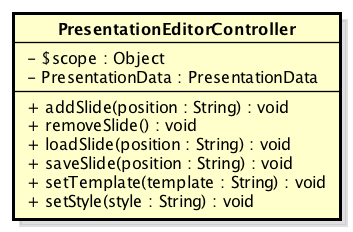
\includegraphics[width=0.5\linewidth]{img/premi_front_end_controllers_presentationeditorcontroller}
	\caption[Premi::Front-End::Controllers::PresentationEditorController]{Premi::Front-End::Controllers::PresentationEditorController}
\end{figure}

	\paragraph{Descrizione}
	Il controller PresentationEditorController si occupa della modifica di una presentazione con i metodi per gestire le slide.
	
	\paragraph{Utilizzo}
	Questa classe viene utilizzata per consentire all'utente di aggiungere o rimuovere una slide dalla presentazione e spostarsi tra di esse. Permette inoltre di impostare lo stile e il template della presentazione.
	
	\paragraph{Attributi}
	\begin{itemize}
		\item \textbf{- PresentationData: PresentationData}:\\
				Campo dati che contiene un riferimento al servizio che si occupa della gestione dei dati e delle impostazioni di una presentazione;
		\item \textbf{\$scope: Object}:\\
				Campo dati contenente un riferimento all'oggetto \$scope creato da Angular, viene utilizzato come mezzo di comunicazione tra il controller e la view. Contiene gli oggetti che definiscono il model dell'applicazione.
	\end{itemize}
	
	\paragraph{Metodi}
	\begin{itemize}
		\item \textbf{addSlide(direction: String)}:\\
				Metodo che aggiunge una slide alla presentazione rispetto alla slide corrente nella posizione indicata da \textit{direction}\footnote{Per \textit{direction} si intende la direzione nella quale si vuole aggiungere o caricare una slide\{up, right, down, left\}};
		\item \textbf{removeSlide()}:\\
				Metodo che rimuove la slide corrente dalla presentazione caricata sul canvas di editing;
		\item \textbf{loadSlide(direction: String)}\\
				Metodo che carica la slide nella posizione indicata da \textit{direction};
		\item \textbf{saveSlide()}\\
				Metodo che salva la slide correntemente caricata sul canvas di editing;
		\item \textbf{setTemplate(template: template)}
				Metodo che imposta il template per la presentazione con quello passato per parametro;
		\item \textbf{setStyle(style: JSON)}
				Metodo che imposta lo stile della presentazione con quello passato per parametro.
	\end{itemize}
	\paragraph{Relazioni con altre classi}
	\begin{itemize}
	  \item OUT: \textbf{PresentationEditorView}:\\
		La vista PresentationEditorView utilizza PresentationEditorController per la gestione delle slide nella composizione e modifica di una presentazione;	
	  \item IN: \textbf{PresentationData}.
	  \item IN: \textbf{SlideEditorView}.
	  \item IN: \textbf{SlideEditorController}.
	\end{itemize}  
\subsubsection{ProjectController}
	\paragraph{Descrizione}
	Il controller ProjectController gestisce il progetto corrente.
	
	\paragraph{Utilizzo}
	Questa classe viene utilizzata per modificare un progetto esistente\footnote{Un progetto vuoto viene creato di default con una presentazione vuota.}.\\
	Permette di aggiungere infografiche, richiamare le funzionalità di modifica di infografiche e della presentazion. Inoltre permette di lanciare la vista di visualizzazione della presentazione.
	\paragraph{Attributi}
	\begin{itemize}
		\item \textbf{-\$scope: Object}:\\
			Campo dati contenente un riferimento all'oggetto \$scope creato da Angular, viene utilizzato come mezzo di comunicazione tra il controller e la view. Contiene gli oggetti che definiscono il model dell'applicazione;
		\item \textbf{-ProjectService: ProjectService}:\\
			Campo dati che contiene un riferimento al servizio che si occupa di reperire le informazioni necessarie al corretto funzionamento della vista ProjectView che rappresenta una sorta di Dashboard di progetto.
	\end{itemize}
	
	\paragraph{Metodi}
	\begin{itemize}
	  \item \textbf{+setPresentation(\textit{id}:Int):void}:\\
		  Metodo che imposta la presentazione identificata da  \textit{id} per la corretta erogazione della presentazione da parte della vista PresentationView;
	  \item \textbf{+getPresentation():JSON}:\\
		  Metodo che restituisce un oggetto JSON contenente un array con tutte le slides della presentazione con le relative coordinate nella presentazione.
		  
	\end{itemize}
	\paragraph{Relazioni con altre classi}
	\begin{itemize}
	  \item OUT: \textbf{ProjectView}:\\
		La vista ProjectView utilizza ProjectController per la gestione reperire ed aggiornare le informazioni di pertinenza del progetto corrente;	
	  \item IN: \textbf{ProjectService}.
		La vista ProjectView utilizza il service ProjectService per reperire ed aggiornare le informazioni di pertinenza del progetto corrente dal back-end.
	\end{itemize}
	
\subsubsection{ProjectsController}
	\paragraph{Descrizione}
	Il controller ProjectsController gestisce i progetti dell' utente corrente.
	
	\paragraph{Utilizzo}
	Questa classe viene utilizzata per visualizzare tutti i progetti dell'utente corrente, lanciarne la modalità di modifica (gestita da ProjectController) e crearne di nuovi.\\
	\paragraph{Attributi}
	\begin{itemize}
		\item \textbf{-\$scope: Object}:\\
			Campo dati contenente un riferimento all'oggetto \$scope creato da Angular, viene utilizzato come mezzo di comunicazione tra il controller e la view. Contiene gli oggetti che definiscono il model dell'applicazione;
		\item \textbf{-ProjectService: ProjectService}
	\end{itemize}
	
	\paragraph{Metodi}
	\begin{itemize}
	  \item \textbf{+setPresentation(\textit{id}:Int):void}:\\
		  Metodo che imposta la presentazione identificata da  \textit{id} per la corretta erogazione della presentazione da parte della vista PresentationView;
	  \item \textbf{+getProject(\textit{id}:Int):JSON}:\\
		  Metodo che restituisce un oggetto JSON contenente un array con la presentazione e tutte le infografiche del progetto identificato da \textit{id}.
		  
	\end{itemize}
	\paragraph{Relazioni con altre classi}
	\begin{itemize}
	  \item OUT: \textbf{ProjectsView}:\\
		La vista ProjectsView utilizza ProjectsController per la gestione reperire ed aggiornare le informazioni di pertinenza dei progetti dell'utente corrente;	
	  \item IN: \textbf{ProjectService}.
		La vista ProjectsView utilizza il service ProjectService per reperire ed aggiornare le informazioni di pertinenza dei progetti dell'utente corrente dall back-end.
	\end{itemize}		
\subsubsection{SearchController}
	\paragraph{Descrizione}
	Il controller SearchController gestisce le funzionalità di ricerca del sistema.
	
	\paragraph{Utilizzo}
	Questa classe viene utilizzata per visualizzare tutti i risultati di ricerca a seguito di una interrogazione da parte di utente qualunque.\\
	\paragraph{Attributi}
	\begin{itemize}
		\item \textbf{-\$scope: Object}:\\
			Campo dati contenente un riferimento all'oggetto \$scope creato da Angular, viene utilizzato come mezzo di comunicazione tra il controller e la view. Contiene gli oggetti che definiscono il model dell'applicazione;
		\item \textbf{-ProjectService: ProjectService}
			Campo dati che contiene un riferimento al servizio che si occupa di gestire le funzionalità di gestione di un progetto nel sistema.
	\end{itemize}
	
	\paragraph{Metodi}
	\begin{itemize}
	  \item \textbf{+searchUsers(\textit{username}:String):JSON}:\\
		  Metodo ritorna un oggetto JSON contenente un array di tutti i progetti dell'utente con username \textit{username};
	  \item \textbf{+searchProject(\textit{name}:String):JSON}:\\
		  Metodo ritorna un oggetto JSON contenente un array di tutti i progetti il cui nome ha un match con \textit{name};
	  \item \textbf{+search(\textit{query}:String):JSON}:\\
		  Metodo ritorna un oggetto JSON contenente un array di tutti i progetti il cui nome ha un match con \textit{name} e dell'utente con username \textit{username};
		  
	\end{itemize}
	\paragraph{Relazioni con altre classi}
	\begin{itemize}
	  \item OUT: \textbf{SearchView}:\\
		La vista SearchView utilizza ProjectsController per la gestione reperire ed aggiornare le informazioni di pertinenza dei progetti che hanno un match con il nome del progetto oppure con lo username dell'utente;	
	  \item IN: \textbf{ProjectService}.
		La vista SearchView utilizza il service ProjectService per reperire ed aggiornare le informazioni di pertinenza dei progetti dal back-end che hanno un match con il nome del progetto oppure con lo username dell'utente proprietario a seguito di un'interrogazione.	
	\end{itemize}		
	
\subsubsection{SignUpController}
	\paragraph{Descrizione}
	Il controller SignUpController gestisce le funzionalità di registrazione di un nuovo utente nel sistema.
	
	\paragraph{Utilizzo}
	Questa classe viene utilizzata per permettere alla view SignUpView di registrare un nuovo utente.\\
	\paragraph{Attributi}
	\begin{itemize}
		\item \textbf{-\$scope: Object}:\\
			Campo dati contenente un riferimento all'oggetto \$scope creato da Angular, viene utilizzato come mezzo di comunicazione tra il controller e la view. Contiene gli oggetti che definiscono il model dell'applicazione;
		\item \textbf{-AuthenticationService: AuthenticationService}:\\
			Campo dati che contiene un riferimento al servizio che si occupa di gestire le funzionalità di autenticazione nel sistema.
	\end{itemize}
	
	\paragraph{Metodi}
	\begin{itemize}
	  \item \textbf{+register(\textit{username}:String,\textit{password}:String):boolean}:\\
		 Metodo che esegue la procedura di registrazione di un nuovo utente con username \textit{username} e password \textit{password} ritornando TRUE se la registrazione è andata a buon fine, FALSE altrimenti.
	  \item \textbf{+registerViaFacebook()(\textit{name}:boolean}:\\
		 Metodo che esegue la procedura di registrazione di un nuovo utente con le API di Facebook ritornando TRUE se la registrazione è andata a buon fine, FALSE altrimenti.
	  \item \textbf{+registerViaGooglePlus()(\textit{query}:boolean}:\\
		 Metodo che esegue la procedura di registrazione di un nuovo utente con le API di Google+ ritornando TRUE se la registrazione è andata a buon fine, FALSE altrimenti.
		  
	\end{itemize}
	\paragraph{Relazioni con altre classi}
	\begin{itemize}
	  \item OUT: \textbf{SignUpView}:\\
		La vista SearchView utilizza ProjectsController per la gestione reperire ed aggiornare le informazioni di pertinenza dei progetti che hanno un match con il nome del progetto oppure con lo username dell'utente;	
	  \item IN: \textbf{AuthenticationService}.
		La vista SignUpView utilizza il service AuthenticationService utilizzare la funzionalità di registrazione del Back-End.	
	\end{itemize}		
	
\subsubsection{SlideEditorController}
	\paragraph{Descrizione}
	Il controller SlideEditorController gestisce le funzionalità di modifica di una slide..
	
	\paragraph{Utilizzo}
	Questa classe viene utilizzata per permettere alla view SignUpView di registrare un nuovo utente.\\
	\paragraph{Attributi}
	\begin{itemize}
		\item \textbf{-\$scope: Object}:\\
			Campo dati contenente un riferimento all'oggetto \$scope creato da Angular, viene utilizzato come mezzo di comunicazione tra il controller e la view. Contiene gli oggetti che definiscono il model dell'applicazione;
		\item \textbf{-SlideService: SlideService}:\\
			Campo dati che contiene un riferimento al servizio che si occupa di gestire le funzionalità di modifica e gestione di una slide.
		\item \textbf{-PresentationService: PresentationService}:\\
			Campo dati che contiene un riferimento al servizio che si occupa di gestire le funzionalità di modifica e gestione di una Presentazione.
	\end{itemize}
	
	\paragraph{Metodi}
	\begin{itemize}
	  \item \textbf{+addObject():Int}:\\
		 Metodo che esegue la procedura di aggiunta di un nuovo componente nella slide corrente mediante una chiamata al service PresentationService ritornando il codice identificativo \textit{id}.
	  \item \textbf{+udpateObject(\textit{id}:String):boolean}:\\
		 Metodo che esegue la procedura di aggiornamento di un componente  identificato da \textit{id} nella slide corrente mediante una chiamata al service PresentationService ritornando TRUE in caso di successo e FALSE altrimenti.\\I valori sono presi dalla variabile \$scope.
	  \item \textbf{+removeObject(\textit{id}:String):boolean}\\
		 Metodo che esegue la rimozione di aggiunta del componente identificato da \textit{id} nella slide corrente mediante una chiamata al service PresentationService ritornando TRUE in caso di successo e FALSE altrimenti.
	  \item \textbf{+saveSlide(\textit{id}:Int):boolean}:\\
		 Metodo che esegue la procedura di salvataggio della slide corrente mediante una chiamata al service PresentationService ritornando TRUE in caso di successo e FALSE altrimenti.
	  \item \textbf{+loadSlide(\textit{id}:Int):boolean}:\\
		 Metodo che esegue la procedura di caricamento della slide corrente mediante una chiamata al service PresentationService ritornando TRUE in caso di successo e FALSE altrimenti.
	  	  
	\end{itemize}
	\paragraph{Relazioni con altre classi}
	\begin{itemize}
	  \item OUT: \textbf{SlideEditorView}:\\
		La vista SlideEditorView utilizza SlideEditorController per la gestione reperire ed aggiornare le informazioni di pertinenza della slide corrente;	
	  \item IN: \textbf{SlideService}.
		La vista SlideEditorView utilizza il service SlideService per recuperare ed aggiornare le informazioni della slide crrente sul Back-End.	
	  \item IN: \textbf{PresentationService}.
		La vista SlideEditorView utilizza il service PresentationService capire la posizione della slide nella presentazione sapendo come aggiornare i suoi indici sincronizzandosi con il Back-End.	
	\end{itemize}		
	
	
% 	SlideService
% PresentationService
% addObject(id)
% removeObject(id)